\documentclass[11pt]{article}

\usepackage{amsmath}
\usepackage{amsfonts} 
\usepackage{amsthm}
\usepackage{blkarray}
\usepackage{caption}
\usepackage{enumitem} 
\usepackage{mathtools}
\usepackage{tikz}
\usepackage[top=2cm,bottom=2cm,left=2cm,right=2cm,marginparwidth=1.75cm]{geometry}
\setlength{\parindent}{0cm}
\newcommand{\R}{\mathbb{R}}
\newcommand\simpleGraph[1]{
  \begin{tikzpicture}[every node/.style={circle,draw}]
    \node (a) at (0,1) {};
    \node (b) at (1,1) {};
    \node (c) at (1,0) {};
    \node (d) at (0,0) {};

    \foreach \from/\to in {#1}
      \draw (\from) -- (\to);
  \end{tikzpicture}\hfil
}
\newcommand\itm[1]{\item[\textbf{#1}]}
\newcommand{\incid}{{-}\!{\bullet}\!{-}}
\newcommand{\n}{\vspace{0.3cm}}

\def\lc{\left\lceil}   
\def\rc{\right\rceil}
\def\lf{\left\lfloor}   
\def\rf{\right\rfloor}

\newtheorem{theorem}{Theorem}

\title{\vspace{-1.0cm}MATH 5707 Homework 2}
\author{Fletcher Gornick}
\date{February 14, 2023}

\begin{document}
\maketitle
\begin{itemize}
  \itm{2.1.6} Show that if \(G\) is a tree with \(\Delta \geq k\), then \(G\) has at least \(k\) vertices of degree one.
  \begin{proof}
    From theorems 1.1 and 2.2, we know \(\displaystyle\sum_{v \in V} d_G(v) = 2\varepsilon = 2\nu - 2.\)
    Now we can let \(\ell\) denote the number of vertices with degree 1 in \(G\).  Without loss of generality, let \(v_1\) be our vertex with \(d_G(v_1) \geq k\).  Let the next \(\ell\) vertices \(v_2,v_3,\hdots,v_{\ell + 1}\) have degree 1, and the remaining \(\nu - \ell - 1\) vertices \(v_{\ell+2}, v_{\ell+3}, \hdots, v_{\nu}\) have degree \(\geq 2\).  This gives us the following inequality,
    \[k + \ell + 2(\nu - \ell - 1) \;\;\leq\;\; d_G(v_1) + \sum_{i=2}^{\ell + 1} d_G(v_i) + \sum_{j=\ell+2}^{\nu} d_G(v_j) \;\;=\;\; \sum_{v \in V} d_G(v) \;\;=\;\; 2\nu - 2.\]
    Simplifying the above inequality gives us \(k - \ell + (2\nu - 2) \leq 2\nu - 2 \iff k \leq \ell\), which gives us our desired result.  Thus, we can conclude that \(G\) must have at least \(k\) vertices of degree 1 if \(\Delta \geq k\).
  \end{proof}
  



  \itm{2.1.12} A saturated hydrocarbon is a molecule \(C_m H_n\) in which every carbon atom has four bonds, every hydrogen atom has one bond, and no sequence of bonds forms a cycle.  Show that for every positive integer \(m\), \(C_m H_n\) can exist only if \(n = 2m + 2\).
  \begin{proof}
    Let \(G = (V, E)\) be a graph of our saturated hydrocarbon, with disjoint vertex sets \(V_1\) and \(V_2\) defined like so:
    \begin{align*}
      V_1 \subset V, \quad V_1 &= \{v \in V \mid v \text{ a carbon atom}\}  \text{ (\(m\) elements)} \\
      V_2 \subset V, \quad V_2 &= \{v \in V \mid v \text{ a hydrogen atom}\}  \text{ (\(n\) elements)} \\
      V_1 \cup V_2 &= V
    \end{align*}

    In order to classify our saturated hydrocarbon \(C_m H_n\) as a molecule, it must be connected.  It's also stated that no bonds form a cycle, making our graph \(G\) a connected acyclic graph, or in other words, a tree.  Under this classification, we can use the following equalities:

    \begin{align*}
      2(m+n) - 2 &= 2\nu - 2              & \text{(\(|V_1| + |V_2| = \nu\))}    \\
                 &= 2\varepsilon          & \text{(Theorem 2.2)}                \\
                 &= \sum_{v \in V} d_G(v) & \text{(Theorem 1.1)}                \\
                 &= \sum_{v_1 \in V_1} d_G(v_1) + \sum_{v_2 \in V_2} d_G(v_2)   \\
                 &= 4m + n.               & \text{(\(d_G(C) = 4, d_G(H) = 1\))} \\
    \end{align*}

    Rearranging terms, we get 
    \[2m + 2n - 2 = 4m + n \quad\iff\quad n = 2m + 2.\]
  \end{proof}
  


  \itm{2.2.2} Let \(G\) be connected and let \(e \in E\).  Show that
    \begin{enumerate}[label=(\alph*)]
      \item \(e\) is in every spanning tree of \(G\) if and only if \(e\) is a cut edge of \(G\);
        \begin{enumerate}
          \item[(\(\Rightarrow\))] If \(e\) is not a cut edge, then \(\omega(G-e) = \omega(G) = 1\), and thus \(G-e\) is connected.  By Corollary 2.4.1, \(G-e\) must contain a spanning tree, so there exists spanning tree not containing \(e\). \n

          \item[(\(\Leftarrow\))] Suppose that \(e\) is a cut edge of \(G\), so \(\omega(G-e) > \omega(G) = 1\), thus \(G-e\) is disconnected.  This means that \(G-e\) cannot have a spanning tree, so it must be the case that \(e\) is in every spanning tree of \(G\). \qed \n
        \end{enumerate}

      \item \(e\) is in no spanning tree of \(G\) if and only if \(e\) is a loop of \(G\).
          \begin{enumerate}
            \item[(\(\Leftarrow\))] A loop is a cycle, so obviously if any graph \(G\) contains loop \(e\), it can't be a tree. \n

            \item[(\(\Rightarrow\))] If \(G\) is connected, and \(e\) is not a loop then there exists a tree containing \(e\). \n\\
              If \(\omega(G - e) > 1\), then \(e\) must be in every spanning tree of \(G\), so assume \(e\) is not a cut edge.\n\\
              If there's a spanning tree \(T\) with \(E(T) \subset E(G)\) not containing \(e\), then we can add \(e\) to \(T\) creating a cycle.  Since \(T + e\) has cycle \(C\), we can simply remove some \(e' \in E(C)\) (\(e' \neq e\)). \n\\
              We still have that every vertex in \(C-e'\) is connected, so \(T + e - e'\) must also still be connected, because the vertices that \(e'\) connected are still connected around our path \(C-e'\). \n\\
              So we've now constructed a tree containing \(e\), meaning (b) must be true. \n
          \end{enumerate}
    \end{enumerate}



  \itm{2.2.3} Show that if \(G\) is loopless and has exactly one spanning tree \(T\), then \(G = T\).
    \begin{proof}
      Suppose \(G \neq T\).  If \(G\) not connected then \(G\) has exactly 0 spanning trees and we're done, so suppose \(G\) connected as well.

      Since \(G \neq T\), there exists some edge \(e \in E(G)\) such that \(e \not\in E(T)\).  Now take \(T+e\).  Obviously \(T+e\) must contain some cycle \(C\) (\(T\) is maximally acyclic), so we can do the same steps outlined in 2.2.2 (b) (\(\Rightarrow\)) to create a new tree containing our edge \(e\), so \(G\) must have at least 2 distinct trees.

      We can now conclude that the contrapositive statement defined above must hold.
    \end{proof}
  



  \itm{2.2.5} Show that \(G\) contains at least \(\varepsilon - \nu + \omega\) distinct cycles.
    \begin{proof}
      Let \(F\) be a spanning forest of \(G\), that is, adding any edge \(e \in E(G)\) not already in \(E(F)\) creates a cycle.  \(\nu(F) = \nu(G)\) obviously, and \(\omega(F) = \omega(G)\) because every connected component of \(G\) must be connected in \(F\), otherwise we can add an edge connecting two components which won't create a cycle, contradicting the fact that \(F\) is a spanning forest.

      Each connected component \(F[V_i]\) of \(F\) must be acyclic (otherwise \(F\) is not acyclic), so \(F[V_i]\) must be a tree.  Therefore \(\varepsilon \left(F[V_i]\right) = |V_i| - 1\), which tells us
      \[\varepsilon(F) = \sum_{i=1}^{\omega} \varepsilon \left(F[V_i]\right) = \sum_{i=1}^{\omega} \left(|V_i| - 1 \right) = \left( \sum_{i=1}^{\omega} |V_i| \right) - \omega = \nu - \omega.\]

      Now, since \(F\) is a maximally acyclic subgraph of \(G\), adding any edge to \(F\) in \(G\) must produce a unique cyle, so there are \(\varepsilon(G) - \varepsilon(F) = \varepsilon - (\nu - \omega) = \varepsilon - \nu + \omega\) distinct cycles.
    \end{proof}
    \newpage
  



  \itm{2.4.1} Using the recursion formula of theorem 2.8, evaluate the number of spanning trees in \(K_{3,3}\).

  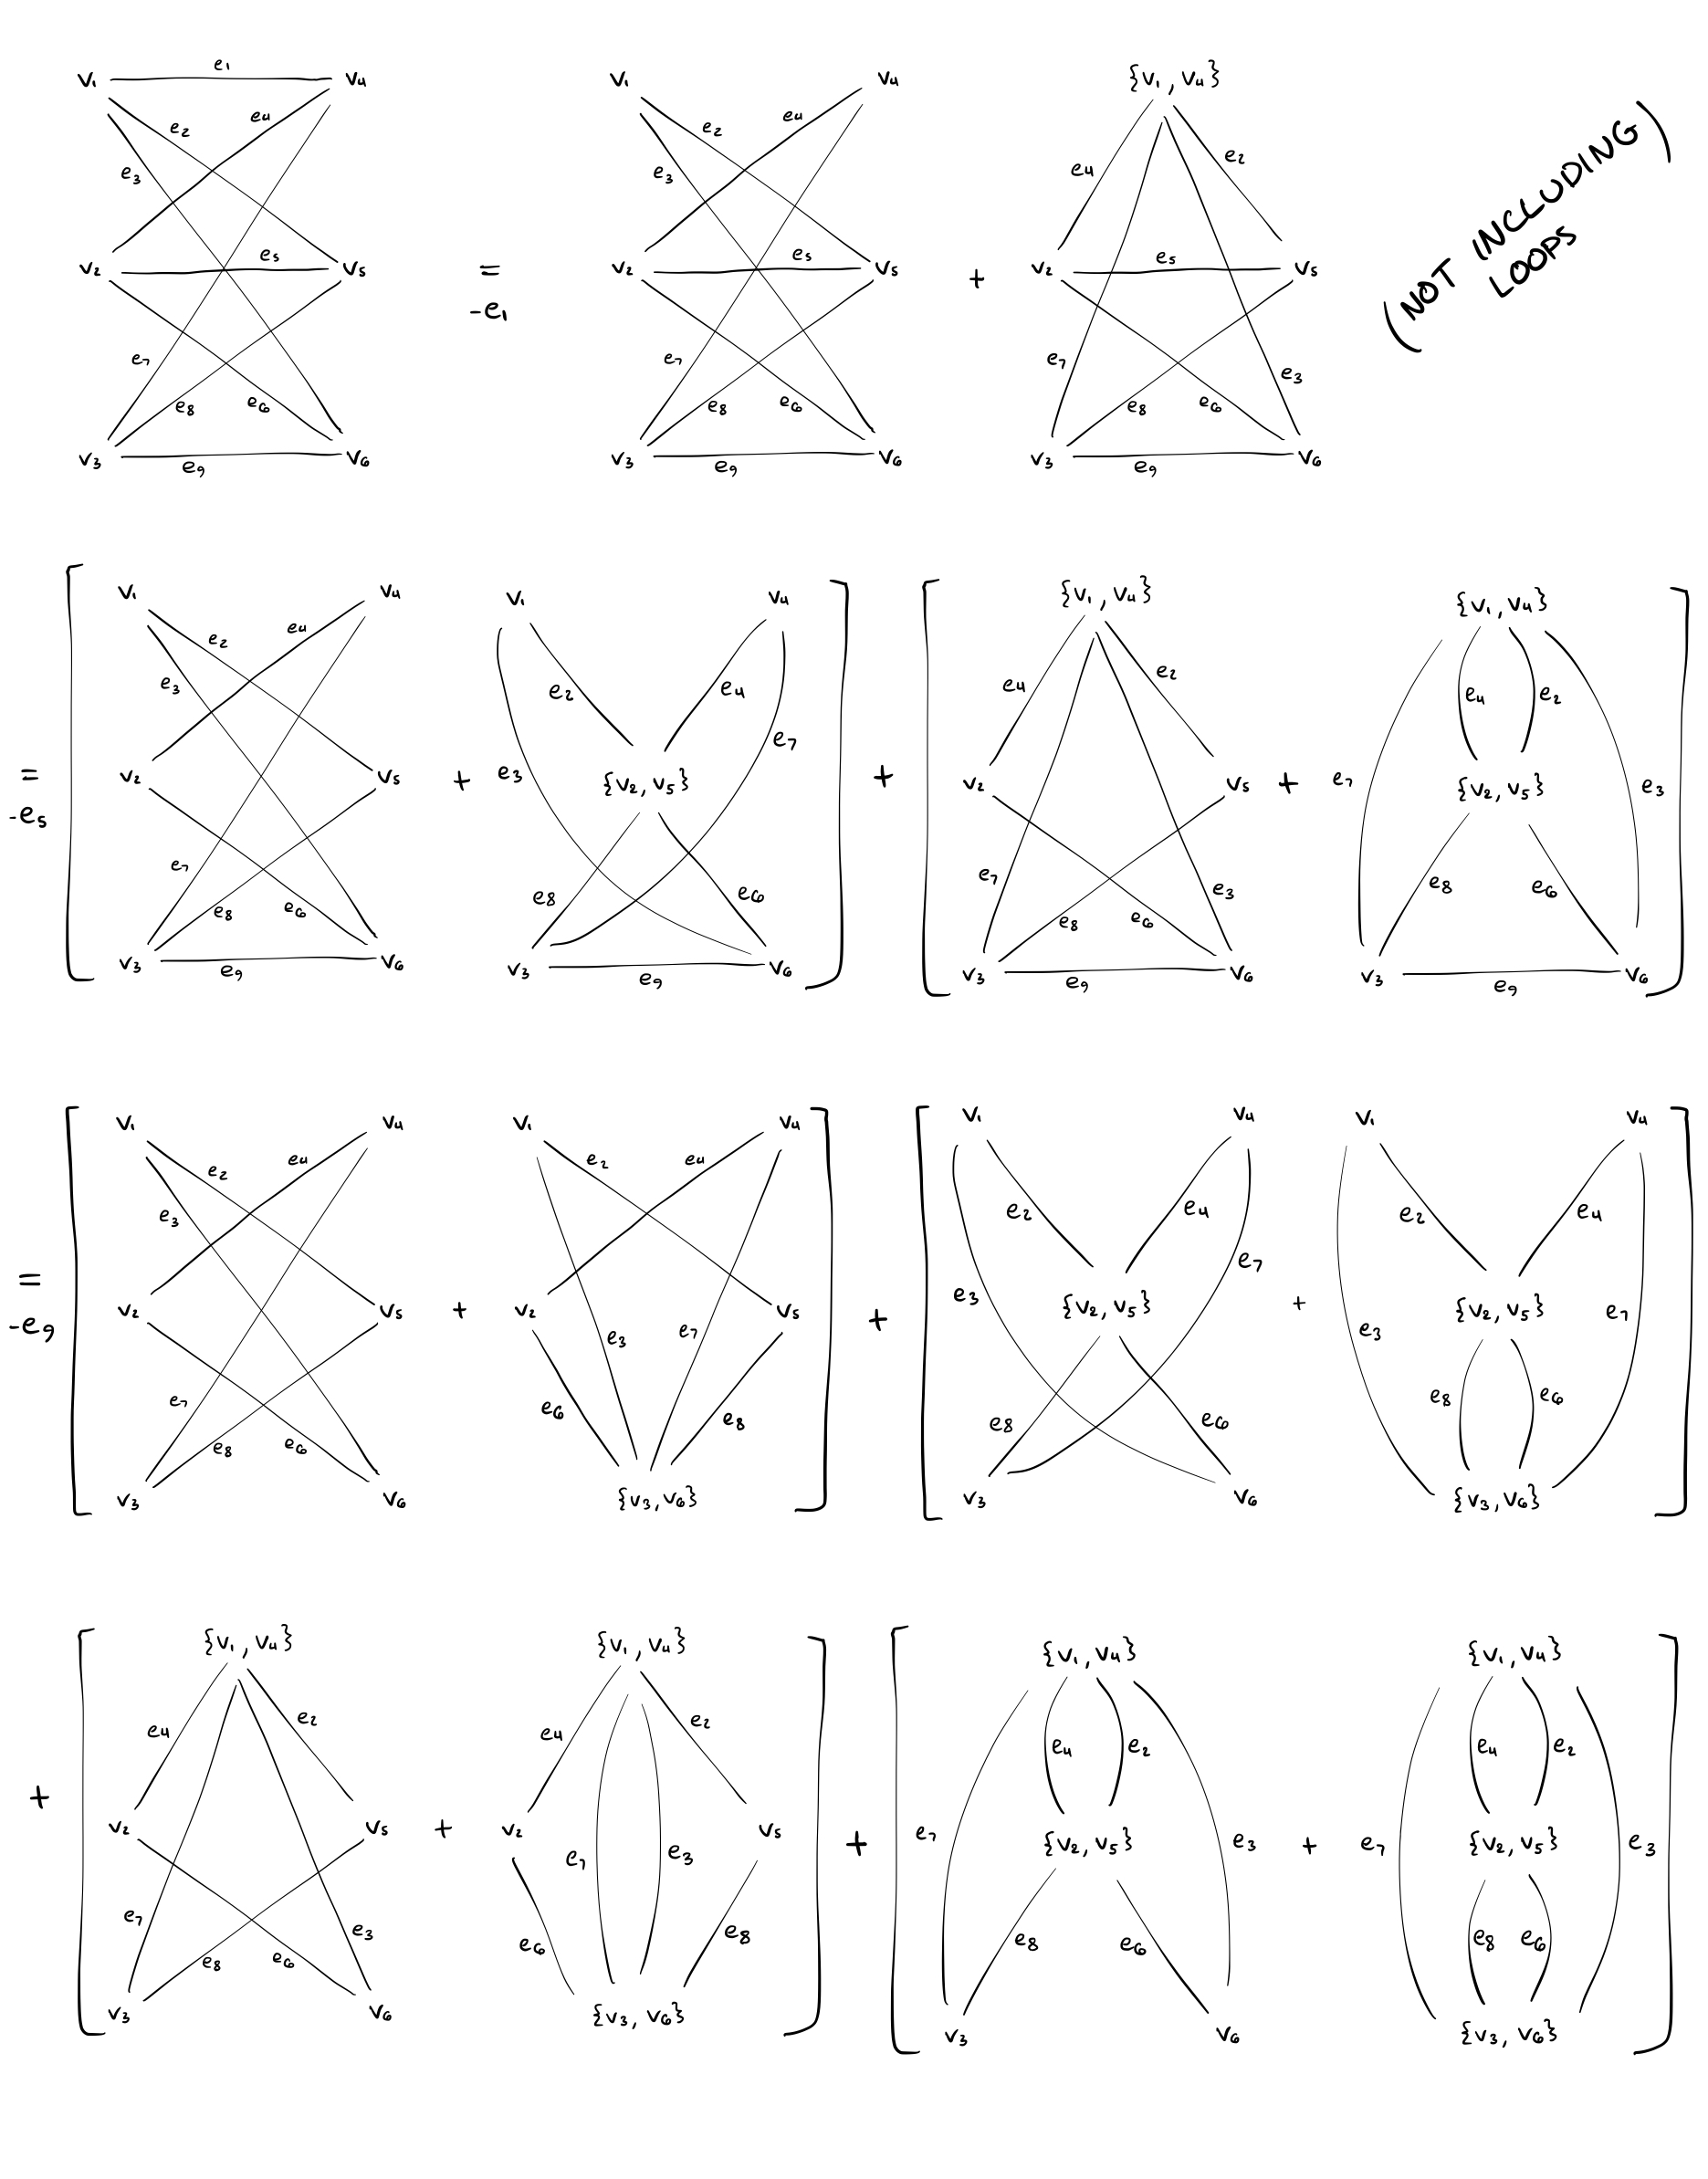
\includegraphics[width=0.95\textwidth]{1.jpeg} \\
  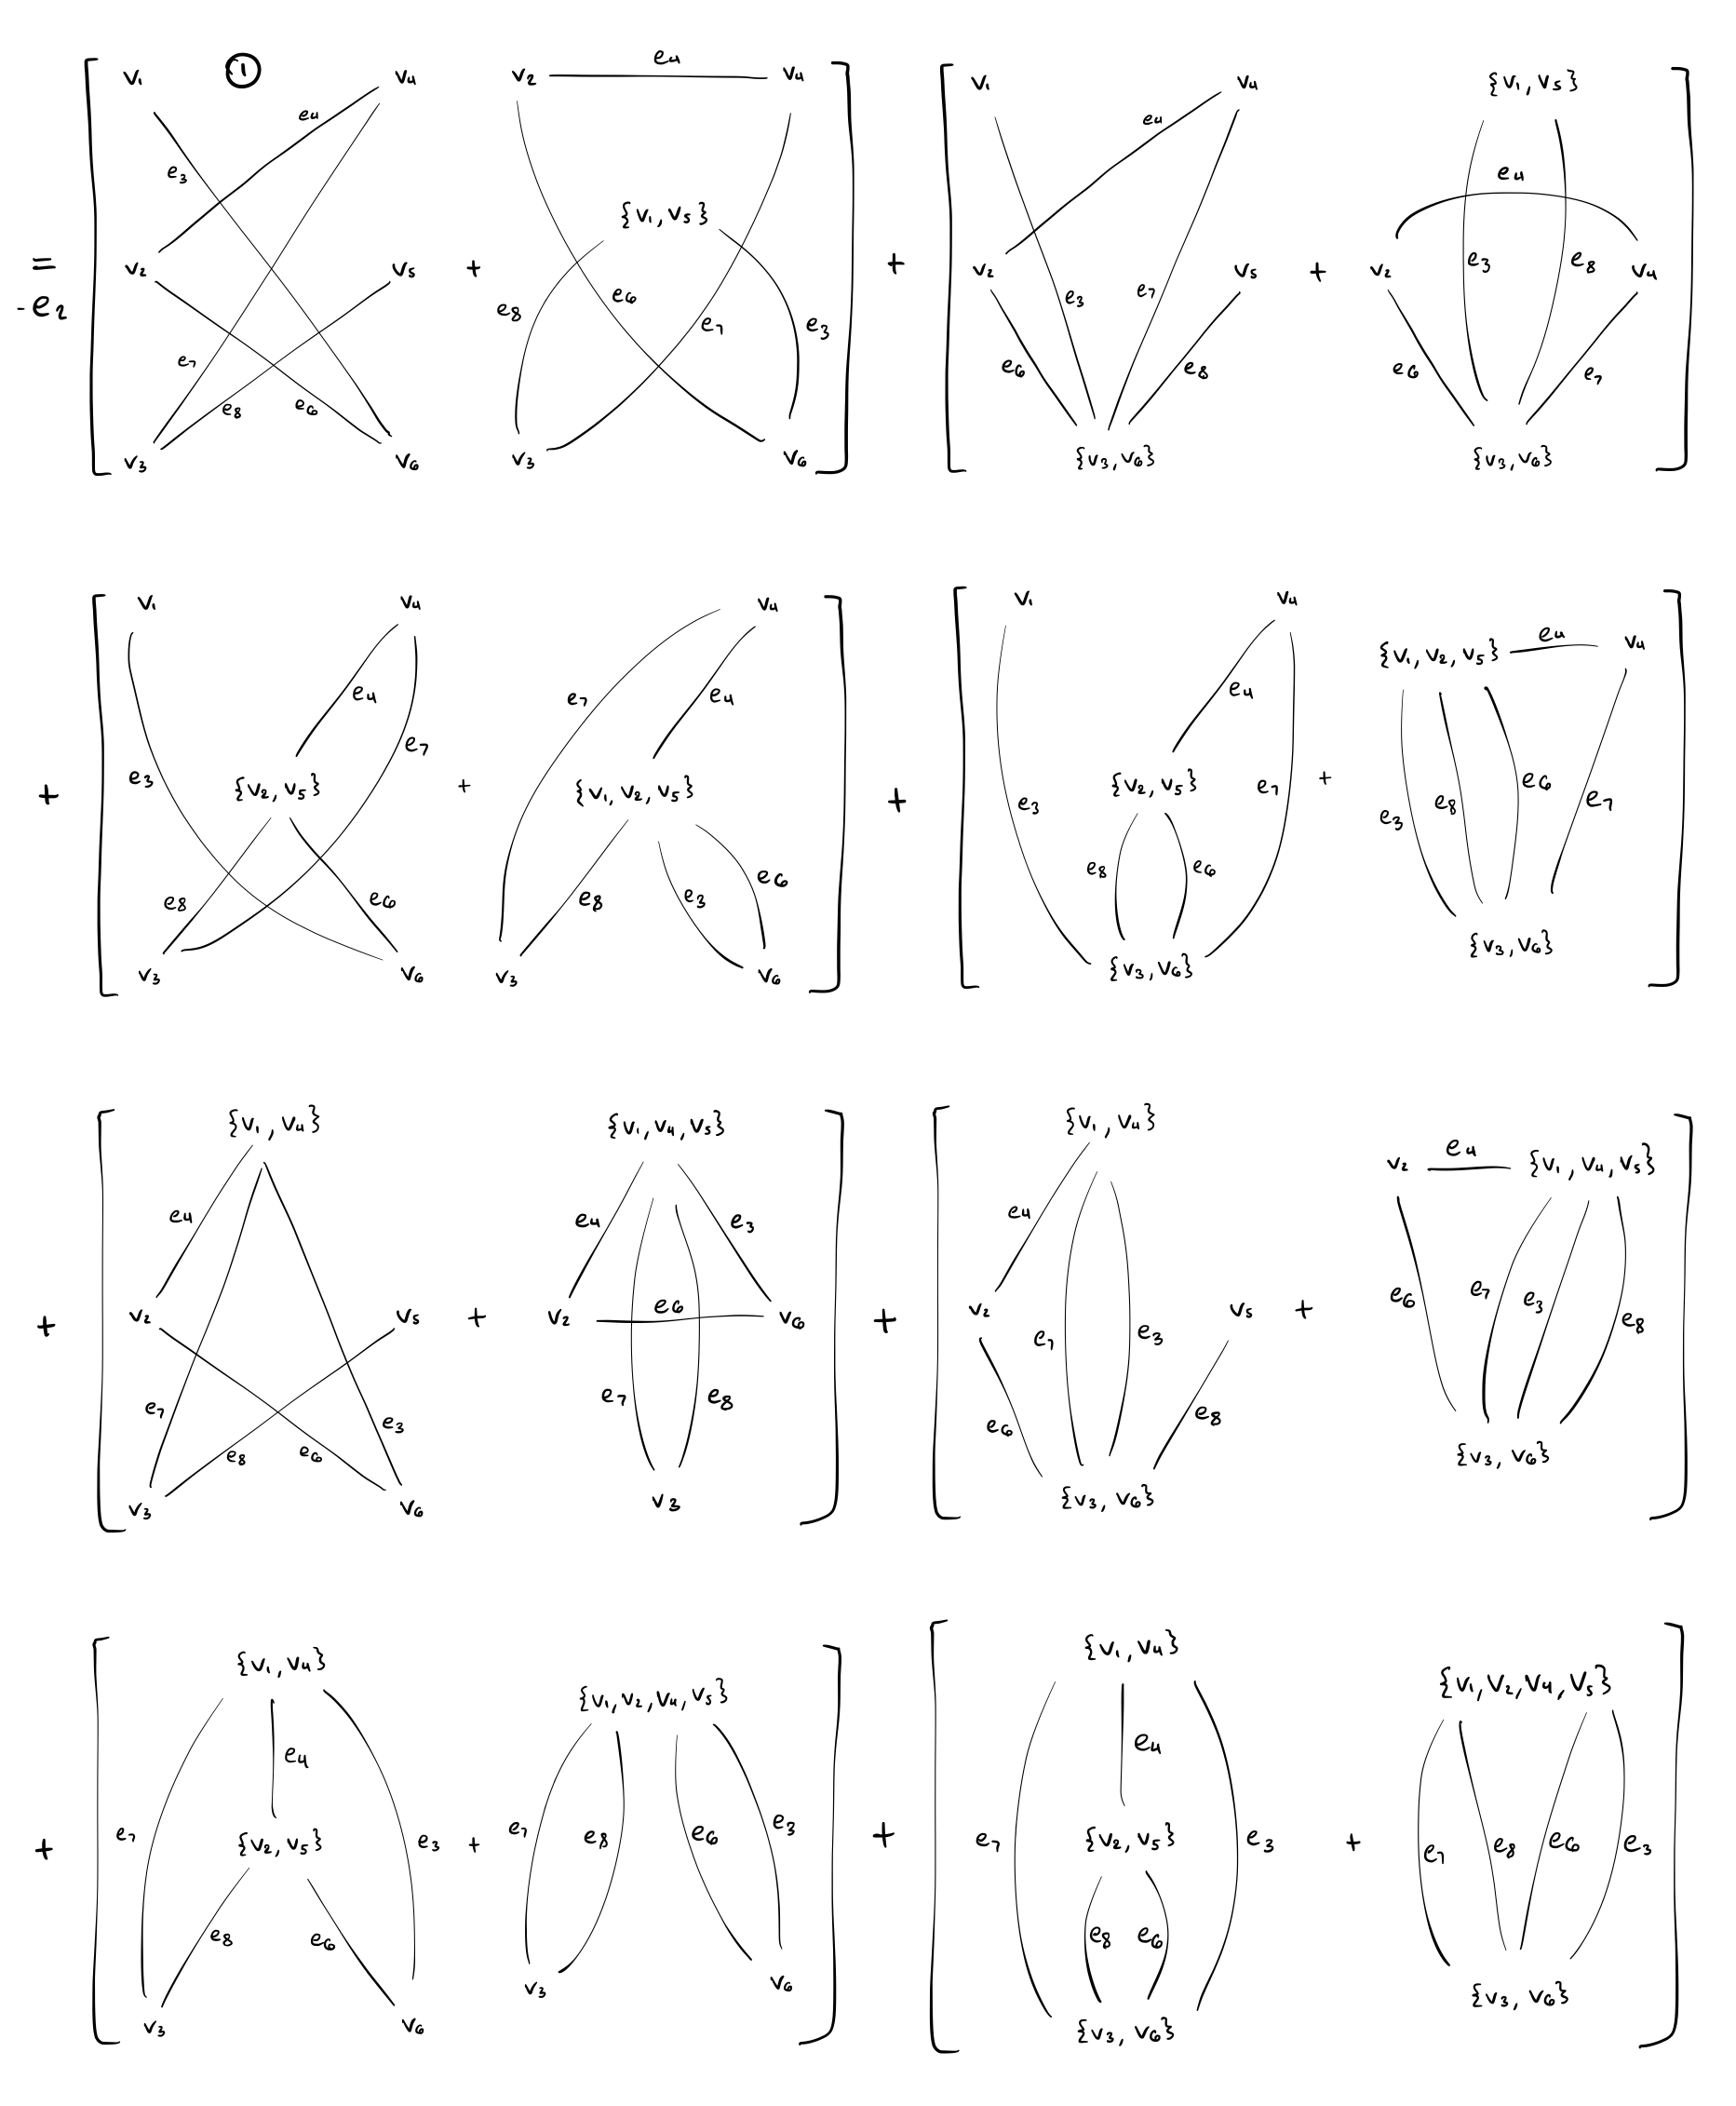
\includegraphics[width=0.95\textwidth]{2.jpeg} \\
  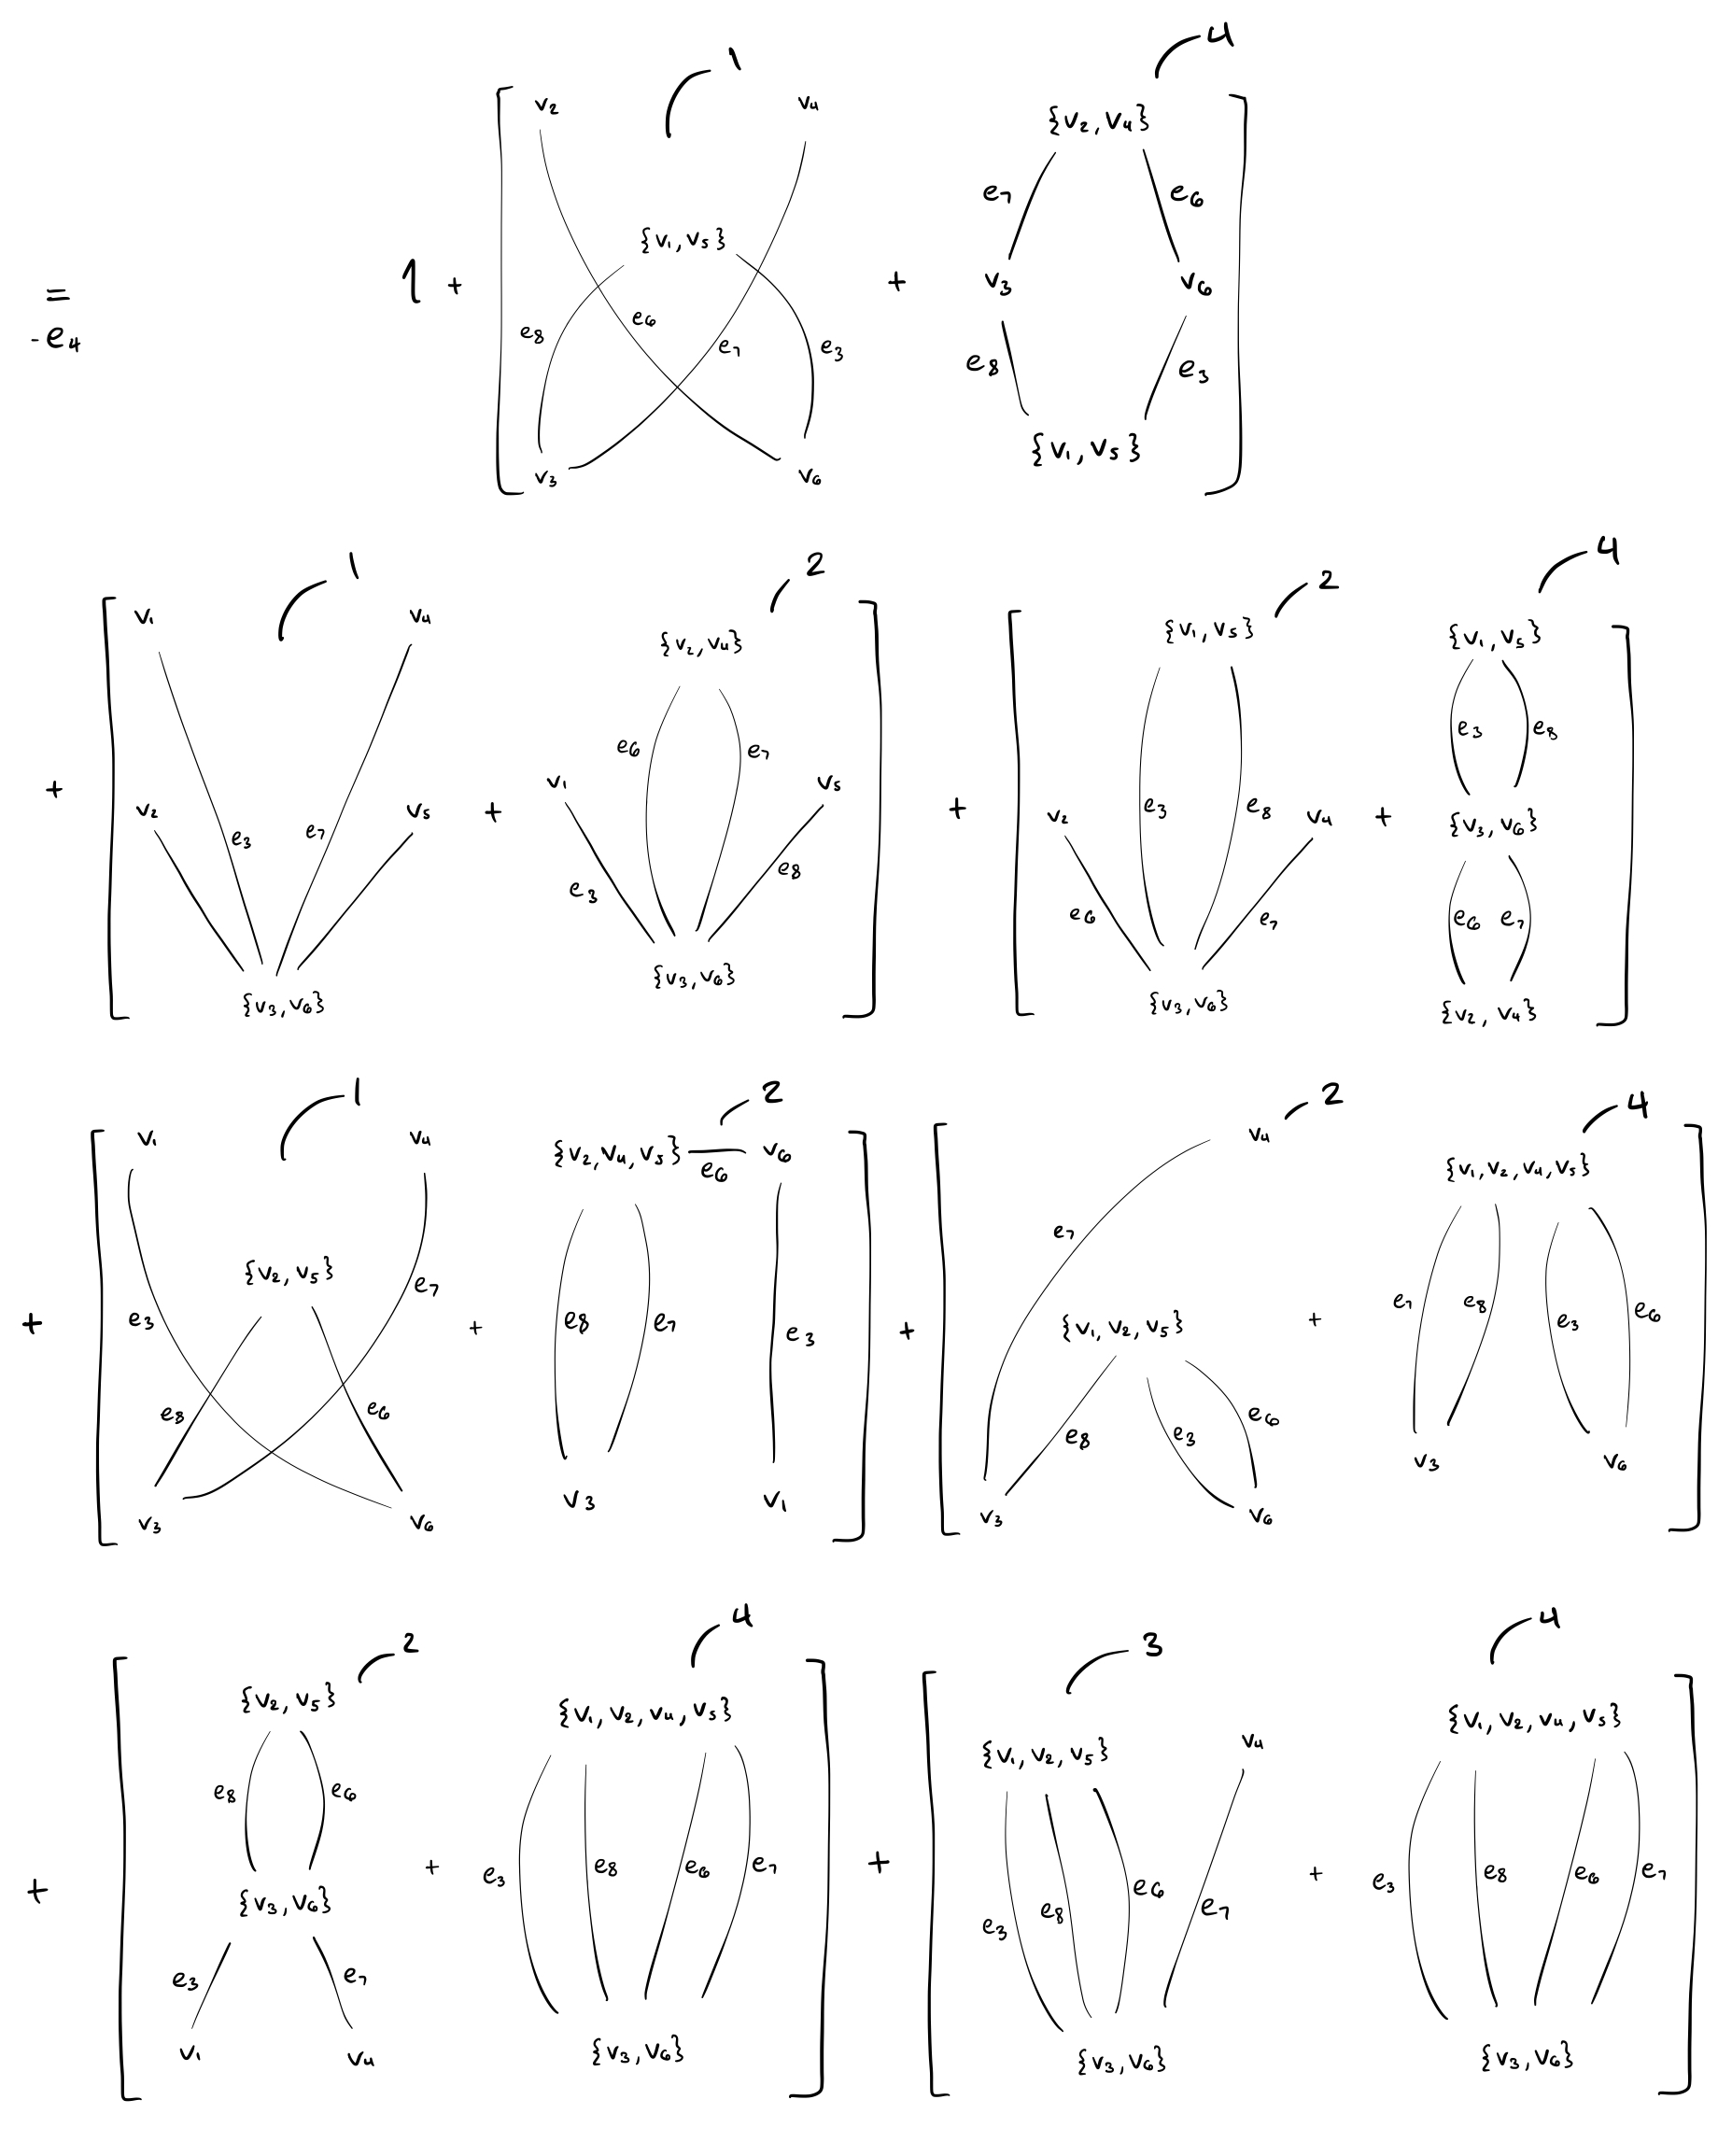
\includegraphics[width=0.95\textwidth]{3.jpeg} \\
  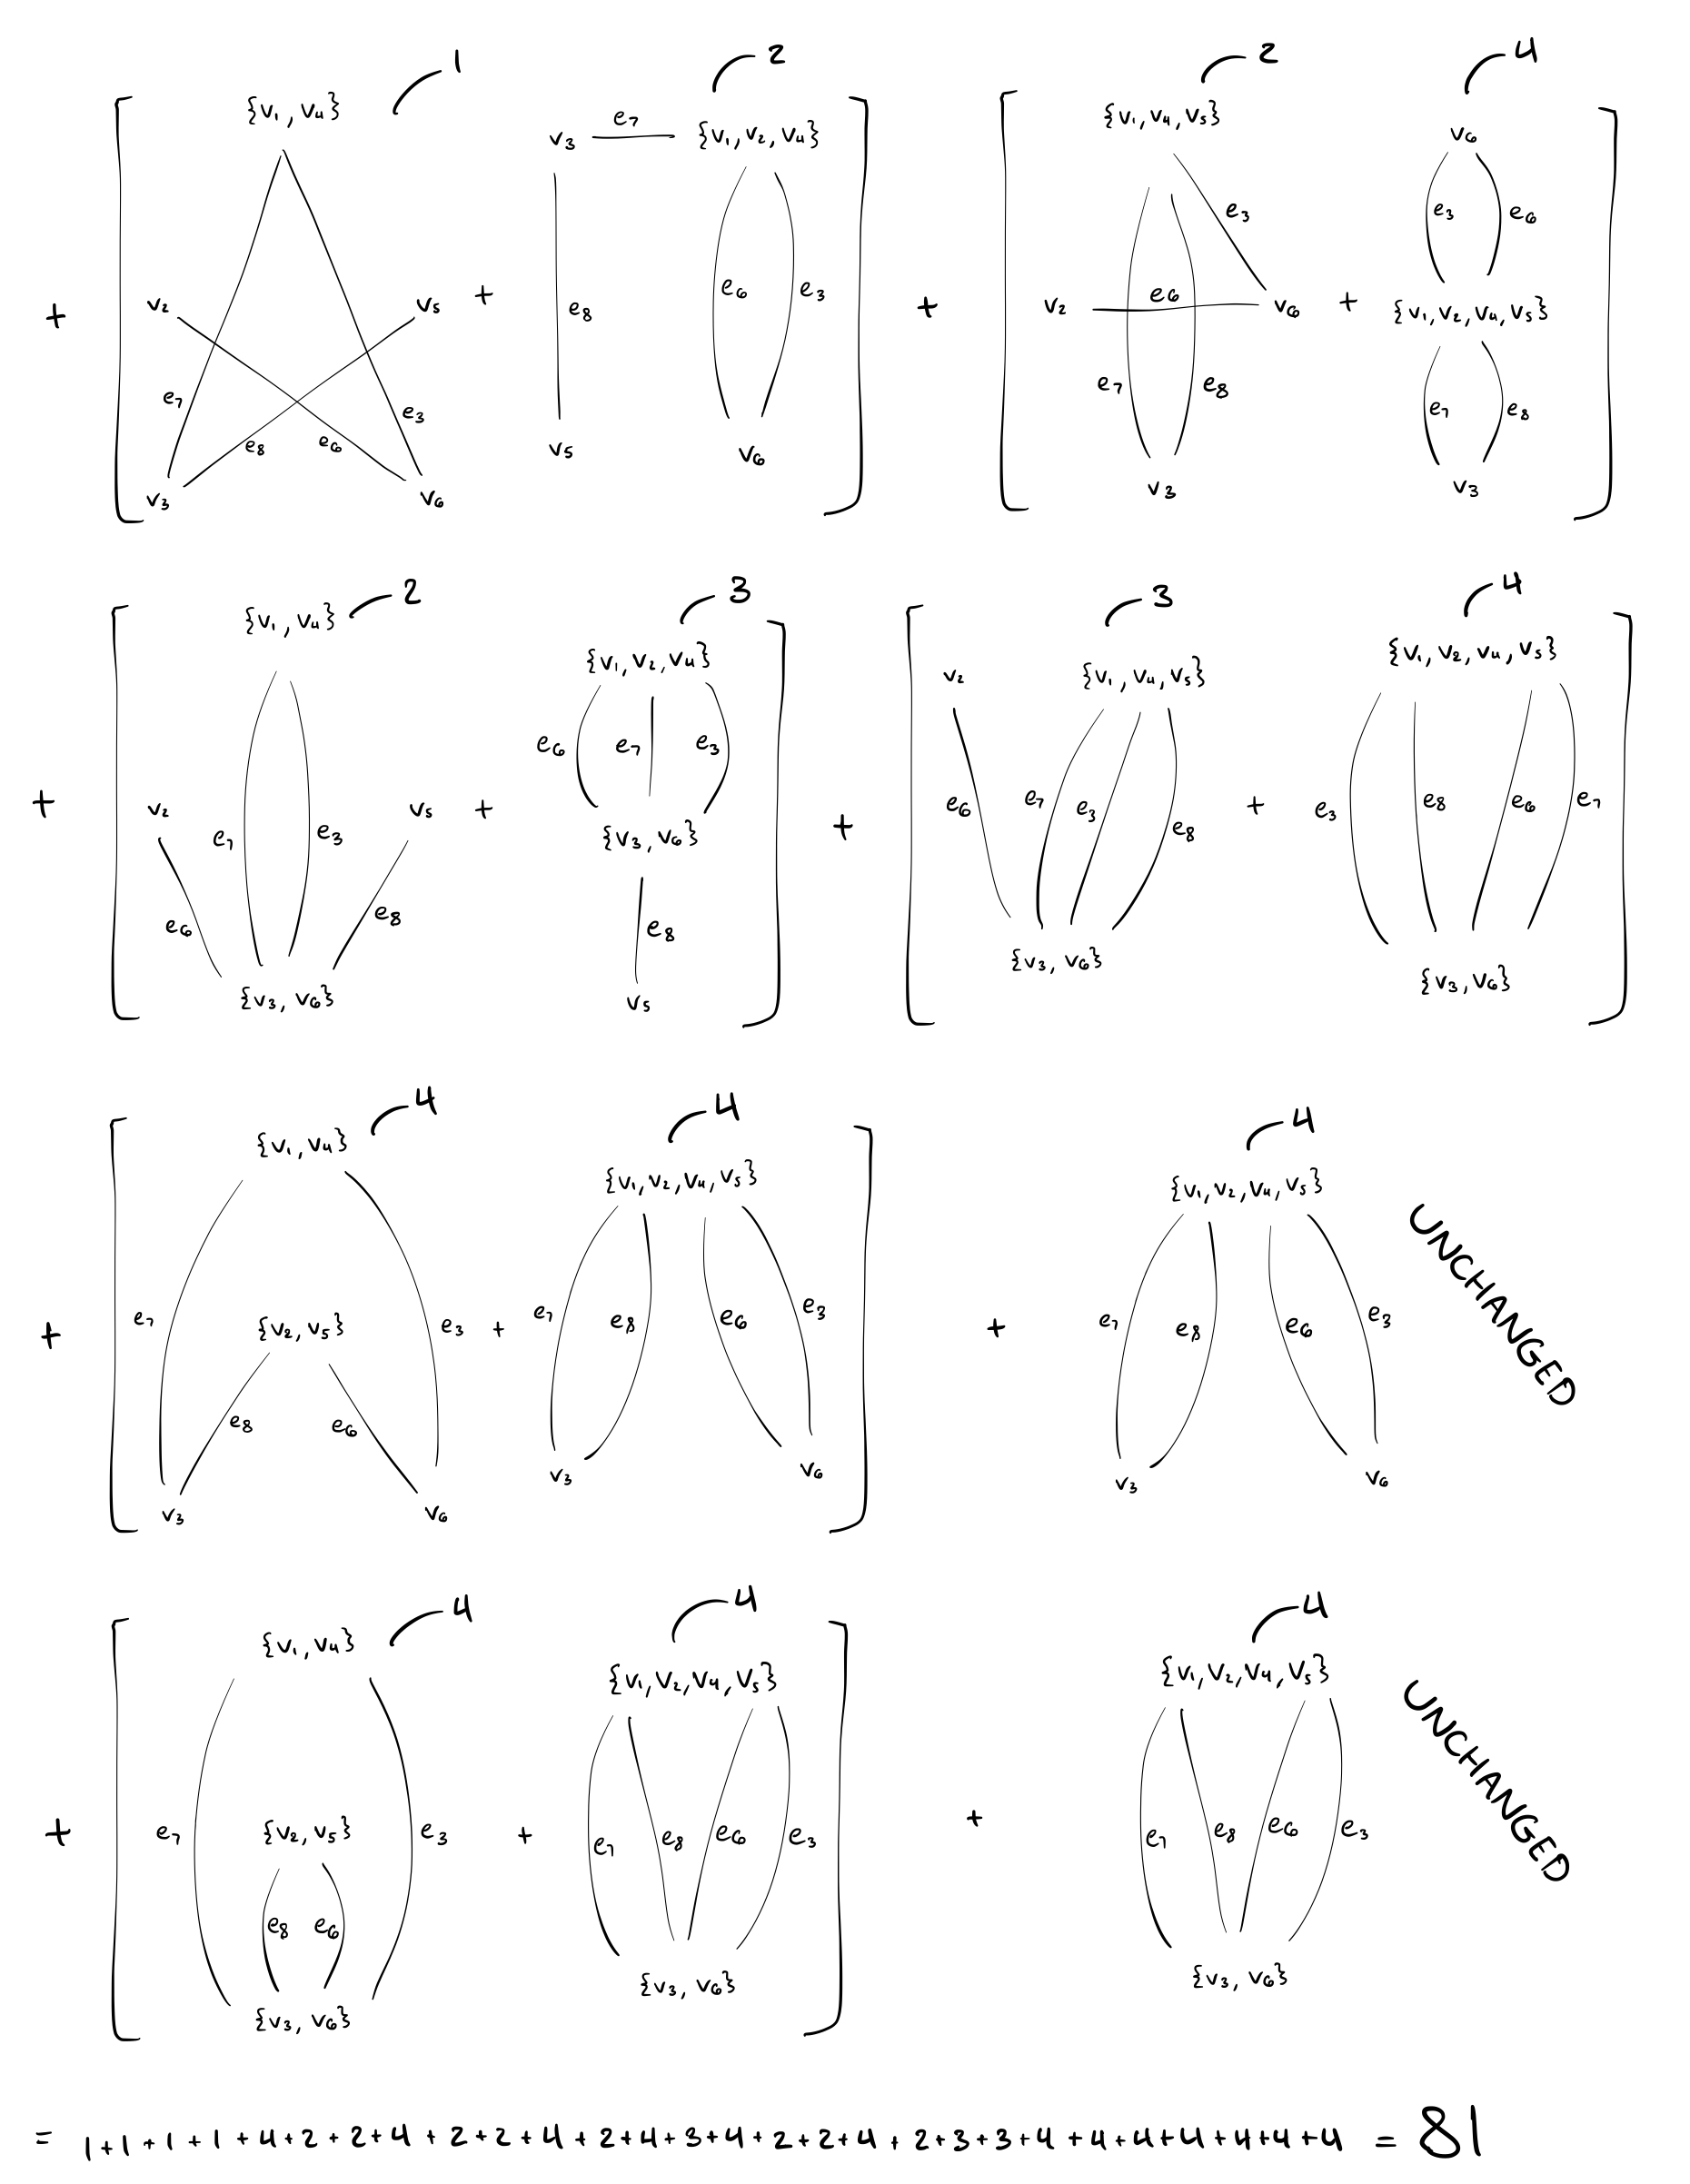
\includegraphics[width=0.95\textwidth]{4.jpeg} \\
  \newpage
  



  \itm{2.4.5} \begin{enumerate}[label=(\alph*)]
      \item Let \(H\) be a graph in which every two adjacent vertices are joined by \(k\) edges and let \(G\) be the underlying simple graph of \(H\).  Show that \(\tau(H) = k^{\nu-1} \tau(G)\).
        \begin{proof}
          From class, we proved \(\tau(G) = \det \left( \overline{L(G)}^{x_0,x_0} \right)\), where \(L(G)\) is defined as follows:
          \[ L_{i,j} =
            \begin{cases}
            \deg(v_i), &\text{ if } i = j, \\
            -1, &\text{ if } i \text{ adjacent to } j, \\
            0, &\text{ otherwise}.
            \end{cases}
          \]
        \(L(G)\) is a \(\nu \times \nu\) matrix, so \(\overline{L(G)}^{x_0,x_0}\) is a \((\nu-1) \times (\nu-1)\) matrix with determinant \(\tau(G)\). \n

        For our new graph \(H\), every adjacent vertex now has \(k\) edges connecting them, whereas there was only 1 for each vertex pair in \(G\) (\(G\) assumed to be simple), so \(d_H(v_i) = k \cdot d_G(v_i)\) for all \(v_i \in V\).  Every off-diagonal entry of \(L(H)\) is also multiplied by \(K\), because every pair of adjacent vertices now have \(k\) edges pairing them.  We now have that 
        \[\overline{L(H)}^{x_0,x_0} = k \cdot \overline{L(G)}^{x_0,x_0},\]\n
        and since \(\overline{L(H)}^{x_0,x_0}\) has \(\nu - 1\) rows and columns, 
        \[\tau(H) = \det \left( \overline{L(H)}^{x_0,x_0} \right) = k^{\nu-1} \cdot \det \left( \overline{L(G)}^{x_0,x_0} \right) = k^{\nu-1} \tau(G).\]
        (Scaling a row by \(k\) multiplies the determinant by \(k\), and we scale \(\nu - 1\) rows.)
        \end{proof}

      \item Let \(H\) be the graph obtained from a graph \(G\) where each edge of \(G\) is replaced by a path of length \(k\).  Show that \(\tau(H) = k^{\varepsilon - \nu + 1} \tau(G)\).
        \begin{proof}
          First, let \(H\) be defined above, and for any edge \(e \in E(G)\), let \(P_e\) be it's corresponding path in \(H\).  There are two cases to consider for each edge \(e\) connecting vertices \(x,y \in G\) when calculating the number of spanning trees of \(H\).  For each of these cases, let \(T\) be any arbitrary spanning tree of \(G\), and let \(T'\) be any one of \(T\)'s corresponding spanning tree in \(H\). \n

          Case 1: \(e \in T\).  In this case, we must have that every edge \(e' \in P_e\) must be in tree \(T'\) of \(H\), otherwise we wouldn't be able to connect \(x\) and \(y\) in \(H\).  If there did happen to exist another path from \(x\) to \(y\), then that path must also exist in \(T\), but that would mean \(T\) contains a cycle which is a contradiction.  So \(e \in T \implies P_e \in T'\). \n

          Case 2: \(e \not\in T\).  In this case, exactly one edge \(e' \in P_e\) must be missing in \(T'\).  If more than one edge was missing in \(P_e\), then \(T'\) would no longer be connected.  If no edges in \(P_e\) are missing in \(T'\), then we would have 2 distinct paths from \(x\) to \(y\) in \(T'\).  \(P_e\) being the first path, and since \(e \not\in T\), there exists path \(P \in T\) connecting \(x\) and \(y\), so we can just concatenate the paths corresponding to each edge in \(P\) to create a new path \(P' \in T'\) connecting \(x\) and \(y\).  So \(e \not\in T \implies \exists! e' \in P_e \mid e' \not\in T'\). \n

          Since \(\varepsilon(T) = \nu - 1\) for each tree \(T\) of \(G\), we have that there are always \(\varepsilon - \nu + 1\) edges missing in \(T\).  This must also be the case for \(T'\) of \(H\), but with the caveat that each edge is missing from a distinct \(k\)-length path \(P_e \in G\). \n

          So there are \(\varepsilon - \nu + 1\) edges missing in \(T'\), each from a distinct path.  From each path there are \(k\) options for which edge to remove.  So for each spanning tree \(T\) of \(G\), there are exactly \(k^{\varepsilon - \nu + 1}\) options for spanning trees in \(H\), and since there are \(\tau(G)\) spanning trees for \(G\), we can conclude that \(\tau(H) = k^{\varepsilon - \nu + 1} \tau(G)\).
        \end{proof}
        

      \item Deduce from (b) that \(\tau(K_{2,n}) = n 2^{n-1}\).
        \begin{proof}
          We can first start with simple complete graph \(K_2\).  Then we can add any \(n-1\) extra edges connecting our two nodes making a multigraph with one edge repeated \(n\) times.  This graph clearly has \(n\) spanning trees (we could also just deduce this by plugging in the formula derived in (a)). \\
          Now, replacing each of these \(n\) edges with paths of length 2, we get another graph with the desired number of spanning trees by the formula derived in (b), this final graph is isomorphic to \(K_{2,n}\), so \(\tau(K_{2,n}) = n2^{n-1}\).
        \end{proof}
    \end{enumerate}
    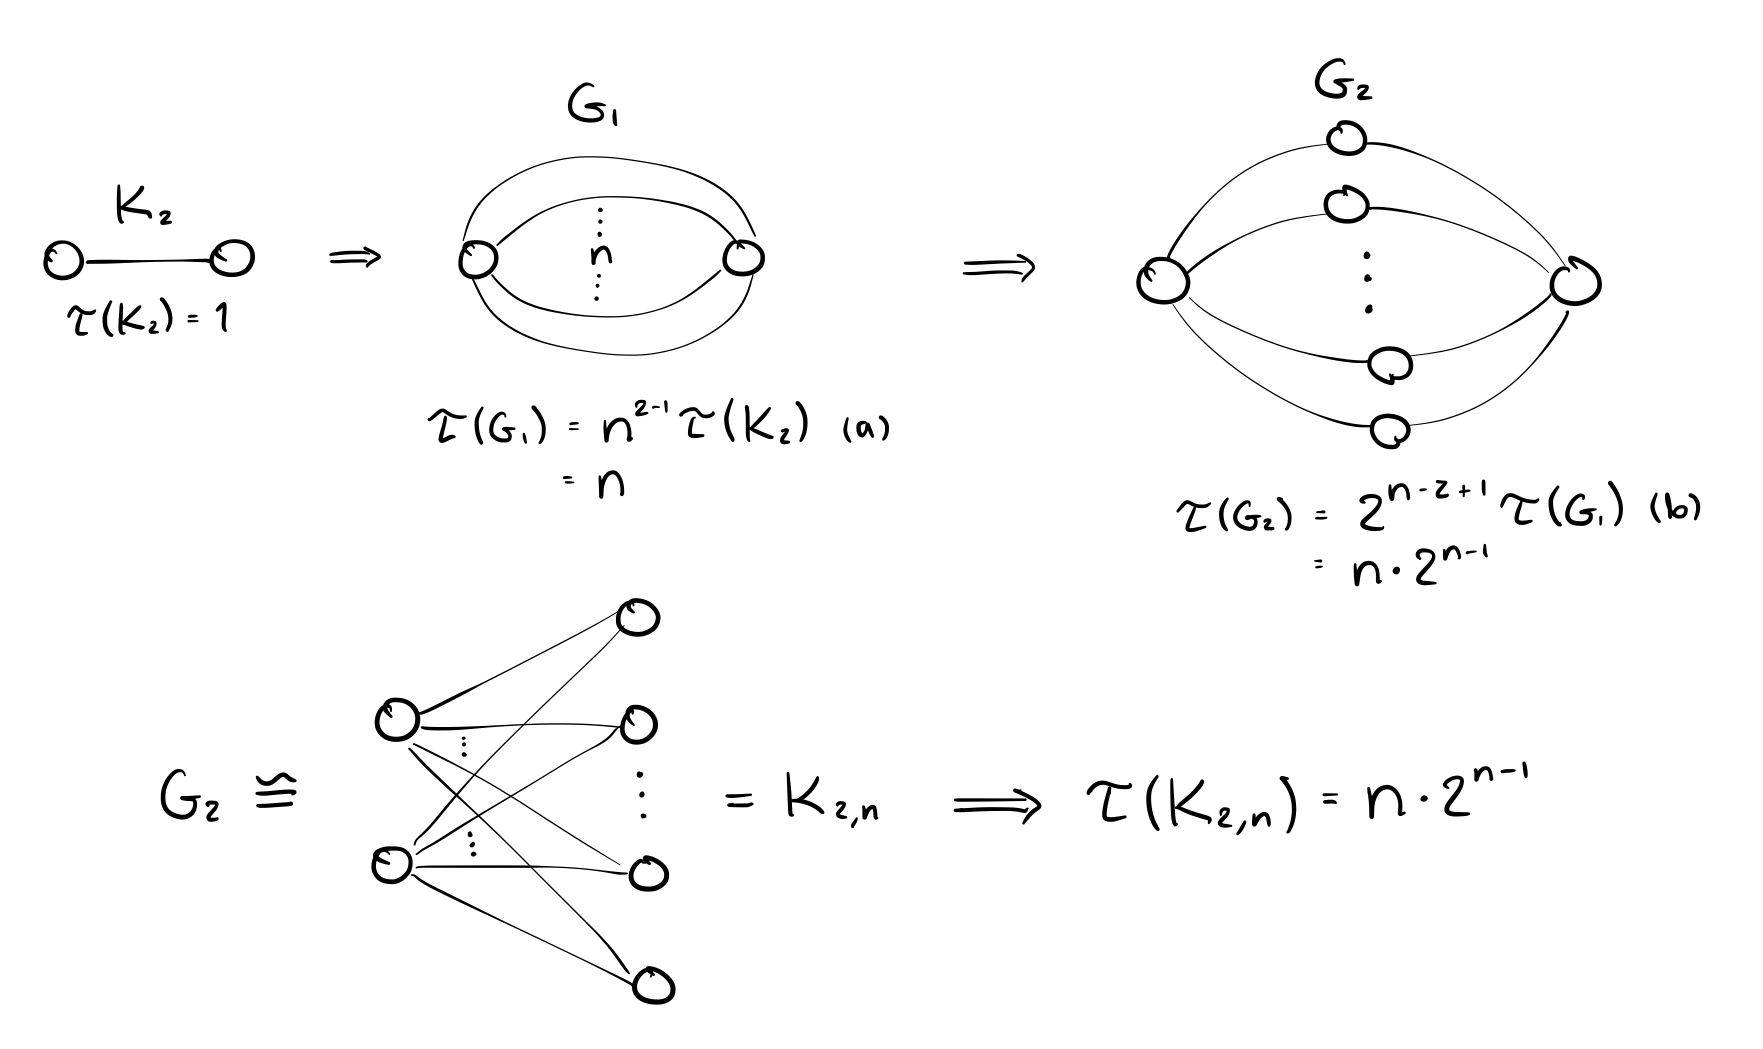
\includegraphics[width=0.90\textwidth]{5.jpeg}



  \itm{2.5.3} Can Kruskal's algorithm be adapted to find
  \begin{enumerate}[label=(\alph*)]
      \item a \textit{maximum}-weight tree in a weighted connected graph? \n\\
        Yes.  Simply just choose each link \(e_i\) so \(w(e_i)\) is as big as possible without creating a cycle instead.  The proof for this is essentially the same as for theorem 2.10. \n

        You could also just negate the weights of \(G\) then negate the weights of the resultant minimum-weight spanning tree to achieve a maximum-weight spanning tree. \n

      \item a minimum-weight maximal forest in a weighted graph? \n\\
        Yes.  You actually don't need to change the algorithm at all to do this.  Since Kruskal's algorithm stops when there's no edge that can be added without creating a cycle, it'll just stop when it finds a minimum-weight maximal forest.

        \begin{proof}
          Suppose it stopped at graph \(G[\{e_1, \hdots, e_{i-1}\}]\) before creating a maximal forest.  Then there would exist edge \(e_i\) not in our result such that \(G[\{e_1, \hdots, e_i\}]\) is acyclic, but that would imply that step 2 of Kruskal's algorithm could have been implemented further, which contradicts the stopping condition outlined in step 3 of Kruskal's algorithm.
        \end{proof}
        
    \end{enumerate}



  \itm{2.5.5} The \textit{tree graph} of a connected graph \(G\) is the graph whose vertices are spanning trees \(T_1, T_2, \hdots, T_{\tau}\) of \(G\), with \(T_i\) and \(T_j\) joined if and only if they have exactly \(\nu-2\) edges in common.  Show that the tree graph of any connected graph is connected.
  \begin{proof}
    Suppose, to the contrary, there's a connected graph that yields a disconnected tree graph.  In other words, for some connected graph \(G\), there exists spanning trees \(T_1, T_2\) such that there's no path from \(T_1\) to \(T_2\) in \(G\)'s tree graph.

    Given spanning tree \(T_1\), choose \(T_2\) to be the spanning tree with the MOST edges in common with \(T_1\) while still being unreachable from \(T_1\) in our tree graph.  Let \(c(T_i, T_j)\) denote the number of edges in common between any spanning trees \(T_i, T_j\).  Clearly \(c(T_1,T_2) < \nu - 2\), otherwise there would be an edge between \(T_1\) and \(T_2\), making them connected.

    Since \(T_1\) and \(T_2\) are distinct trees, we know there's an edge \(e_1 \in T_1\) not in \(T_2\).  And since \(T_2\) is maximally acyclic, \(T_2 + e_1\) must contain some cycle \(C\).  Since \(T_1\) has no cycles, there must exist an edge \(e_2 \in C\) such that \(e_2 \not\in T_1\).

    Take new tree \(T_3 = (T_2 + e_1) - e_2\) (2.2.2 (b) \((\Rightarrow)\) shows why this is a tree).  Since \(e_2 \not\in T_1\), we know that removing it doesn't change the value of \(c(T_1,T_3)\), but adding \(e_1\) to \(T_3\) increments the number of common edges by one, so
    \[c(T_1,T_3) = c(T_1,T_2) + 1,\]
    Which contradicts our assumption that \(c(T_1,T_2)\) is the max.  Therefore the tree graph of any connected graph is connected.
  \end{proof}
  



\end{itemize}

\end{document}
